\documentclass[12pt,a4paper]{article}
\usepackage[utf8]{vietnam}
\usepackage{amsmath,amssymb}
\usepackage{geometry}
\geometry{top=1.2cm,bottom=1.0cm,left=1.3cm,right=1.3cm,headheight=26pt,headsep=10pt,footskip=14pt}
\usepackage{tikz}
\usepackage{xcolor}
\usepackage{enumerate}
\usepackage{graphicx}
\usepackage[version=4]{mhchem}
\usepackage{fancyhdr}
\usepackage{ex_test}

\renewcommand{\baselinestretch}{0.92}
\setlength{\parskip}{0pt}

\definecolor{hfRed}{RGB}{211,47,47}
\definecolor{hfGreen}{RGB}{139,195,144}

\providecommand{\False}{}

\pagestyle{fancy}
\fancyhf{}
\fancyhead[L]{\small\itshape\color{hfRed} Tài liệu lưu hành nội bộ}
\fancyhead[R]{\small\itshape\color{hfRed} Thầy \textbf{TRẦN VĂN THẠNH} - 0777.470.803}
\renewcommand{\headrulewidth}{0.8pt}
\renewcommand{\headrule}{\hbox to\headwidth{\color{hfGreen}\leaders\hrule height \headrulewidth\hfill}}

\fancyfoot[L]{\small\itshape\color{hfRed} CS1: 6/15 Nguyễn Hoàng, P. Kim Long, TP Huế \quad|\quad CS2: 24 Đặng Thái Thân, TP Huế}
\fancyfoot[R]{\small\bfseries\color{hfRed} Trang \thepage}
\renewcommand{\footrulewidth}{0.8pt}
\renewcommand{\footrule}{\hbox to\headwidth{\color{hfGreen}\leaders\hrule height \footrulewidth\hfill}}

\fancypagestyle{firstpage}{
  \fancyhf{}
  \renewcommand{\headrulewidth}{0pt}
  \fancyfoot[L]{\small\itshape\color{hfRed} CS1: 6/15 Nguyễn Hoàng, P. Kim Long, TP Huế \quad|\quad CS2: 24 Đặng Thái Thân, TP Huế}
  \fancyfoot[R]{\small\bfseries\color{hfRed} Trang \thepage}
  \renewcommand{\footrulewidth}{0.8pt}
  \renewcommand{\footrule}{\hbox to\headwidth{\color{hfGreen}\leaders\hrule height \footrulewidth\hfill}}
}

\begin{document}
\thispagestyle{firstpage}

\noindent
\begin{minipage}[t]{0.44\textwidth}
	\centering\fontsize{10pt}{12pt}\selectfont
	\textbf{SỞ GIÁO DỤC VÀ ĐÀO TẠO THỪA THIÊN HUẾ}\\
	\textbf{ĐỀ CHÍNH THỨC}\\
	\textit{(Đề thi có 04 trang)}
\end{minipage}\hfill
\begin{minipage}[t]{0.54\textwidth}
	\centering\small
	\textbf{ĐỀ KIỂM TRA ĐỊNH KỲ CHƯƠNG 2 (CARBOHYDRATE)}\\
	\textbf{MÔN: HOÁ HỌC -- LỚP 12}\\
	\textit{Thời gian làm bài: 50 phút (không kể thời gian phát đề)}\\
	\fbox{\textbf{MÃ ĐỀ: 105}}
\end{minipage}

\smallskip
\noindent\hrulefill
\smallskip

\noindent\textbf{Họ, tên thí sinh:} \dotfill\ \textbf{Lớp:} \dotfill\ \textbf{Số báo danh:} \dotfill

\smallskip
\noindent\textit{(Cho biết nguyên tử khối: H = 1; C = 12; N = 14; O = 16; Na = 23; K = 39; Cu = 64; Ag = 108).}

\vspace{0.2cm}
\noindent
\textbf{PHẦN I (4,5 điểm -- 18 câu): Câu trắc nghiệm nhiều phương án lựa chọn.}\\
\textit{Thí sinh trả lời từ câu 1 đến câu 18. Mỗi câu hỏi thí sinh chỉ chọn một phương án.}

\Opensolutionfile{ans}[ans-de05hs]

\begin{ex}
Saccharose và fructose đều thuộc loại
\choice
{monosaccharide.}
{disaccharide.}
{polysaccharide.}
{carbohydrate.}
\loigiai{}
\end{ex}

\begin{ex}
Một chất khi thủy phân trong môi trường acid, đun nóng \textbf{không} tạo ra glucose. Chất đó là
\choice
{tinh bột.}
{saccharose.}
{cellulose.}
{tripalmitin.}
\loigiai{}
\end{ex}

\begin{ex}
(SBT -- CTST). Carbohydrate nào sau đây là thành phần chính của mật ong?
\choice
{Glucose.}
{Maltose.}
{Saccharose.}
{Fructose.}
\loigiai{}
\end{ex}

\begin{ex}
(SBT -- KNTT). Saccharose thường được tìm thấy trong loại thực vật nào sau đây?
\choice
{Cây đậu nành.}
{Cây lúa mì.}
{Cây mía.}
{Cây cà phê.}
\loigiai{}
\end{ex}

\begin{ex}
(SBT -- KNTT). Công thức phân tử của saccharose là
\choice
{$\ce{C5H10O5}$.}
{$\ce{C6H12O6}$.}
{$\ce{C12H22O11}$.}
{$(\ce{C6H10O5})_n$.}
\loigiai{}
\end{ex}

\begin{ex}
(SBT -- KNTT). Tinh bột và cellulose đều là
\choice
{disaccharide.}
{monosaccharide.}
{polysaccharide.}
{oligosaccharide.}
\loigiai{}
\end{ex}

\begin{ex}
(SBT -- KNTT). Phản ứng màu với dung dịch iodine là tính chất của chất nào sau đây?
\choice
{Glucose.}
{Fructose.}
{Saccharose.}
{Tinh bột.}
\loigiai{}
\end{ex}

\begin{ex}
Glucose có thể lên men tạo lactic acid có trong sữa chua qua phản ứng nào sau đây?
\choice
{$2\ce{C6H12O6 + Cu(OH)2 -> (C6H11O6)2Cu + 2H2O}$}
{$\ce{C6H12O6} \xrightarrow{\text{enzyme}} 2\ce{C2H5OH + 2CO2}$}
{$\ce{C6H12O6} \xrightarrow{\text{enzyme}} 2\ce{CH3CH(OH)COOH}$}
{$\ce{CH2OH[CHOH]4CHO + Br2 + H2O} \xrightarrow{t^\circ} \ce{CH2OH[CHOH]4COOH + 2HBr}$}
\loigiai{}
\end{ex}

\begin{ex}
(SGK 12 -- CTST). Cho các carbohydrate sau: glucose, fructose, saccharose và maltose. Số carbohydrate có khả năng mở vòng trong dung dịch nước là
\choice
{1.}
{2.}
{3.}
{4.}
\loigiai{}
\end{ex}

\begin{ex}
Công thức cấu tạo dạng mạch vòng $\beta$-fructose là:
\begin{center}
\begin{tabular}{cccc}
\textbf{A} & \textbf{B} & \textbf{C} & \textbf{D} \\
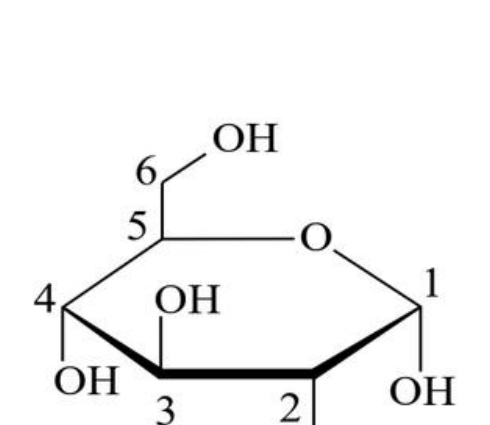
\includegraphics[width=3.2cm]{images_crop_de05/cau10_opt_A.png} &
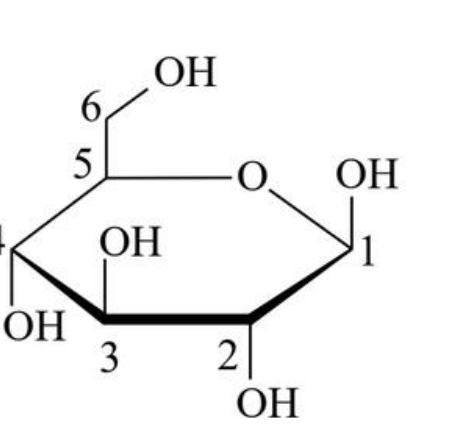
\includegraphics[width=3.2cm]{images_crop_de05/cau10_opt_B.png} &
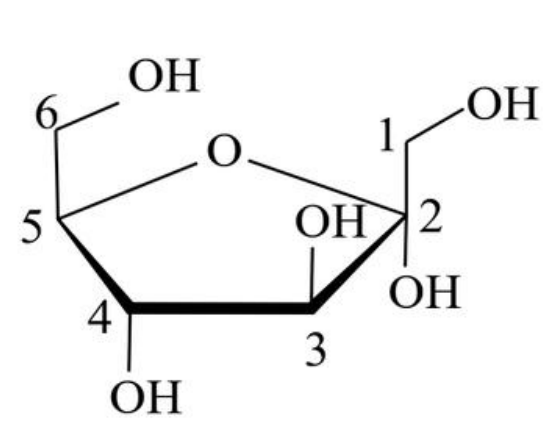
\includegraphics[width=3.2cm]{images_crop_de05/cau10_opt_C.png} &
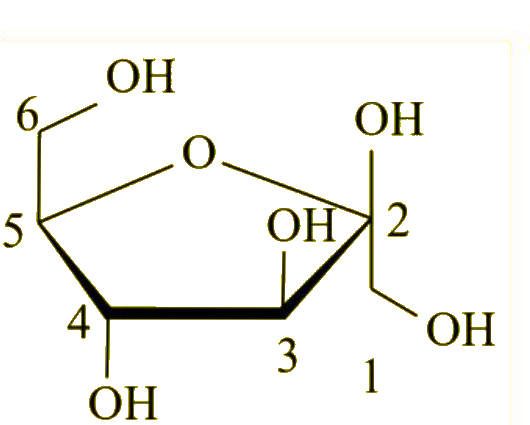
\includegraphics[width=3.2cm]{images_crop_de05/cau10_opt_D.png}
\end{tabular}
\end{center}
\choice
{Hình A.}
{Hình B.}
{Hình C.}
{Hình D.}
\loigiai{}
\end{ex}

\begin{ex}
Mô tả nào dưới đây \textbf{không} đúng với glucose?
\choice
{Chất rắn, khó tan trong nước và có vị ngọt.}
{Có mặt trong hầu hết các bộ phận của cây, nhất là trong quả chín.}
{Còn có tên gọi là đường nho.}
{Có 80-130 mg/dL trong máu người trưởng thành, khỏe mạnh và lúc đói.}
\loigiai{}
\end{ex}

\begin{ex}
Cho các tính chất sau: (1) có vị ngọt, (2) dễ tan trong nước, (3) có phản ứng tráng bạc, (4) bị thủy phân trong môi trường acid, (5) hòa tan $\ce{Cu(OH)2}$ thành dung dịch màu xanh lam.\\
Số tính chất đúng với saccharose là
\choice
{4.}
{3.}
{5.}
{2.}
\loigiai{}
\end{ex}

\begin{ex}
Nhận định sai là
\choice
{Phân biệt glucose và saccharose bằng phản ứng tráng gương.}
{Phân biệt tinh bột và cellulose bằng $\ce{I2}$.}
{Phân biệt saccharose và glycerol bằng $\ce{Cu(OH)2}$.}
{Phân biệt tinh bột và saccharose bằng $\ce{I2}$.}
\loigiai{}
\end{ex}

\begin{ex}
(SBT -- CTST). Hầu hết những phản ứng sinh hoá xảy ra nhờ sự xúc tác của các enzyme. Biểu đồ dưới đây thể hiện tốc độ của một phản ứng sinh hoá do enzyme X làm chất tác theo nhiệt độ:
\begin{center}
	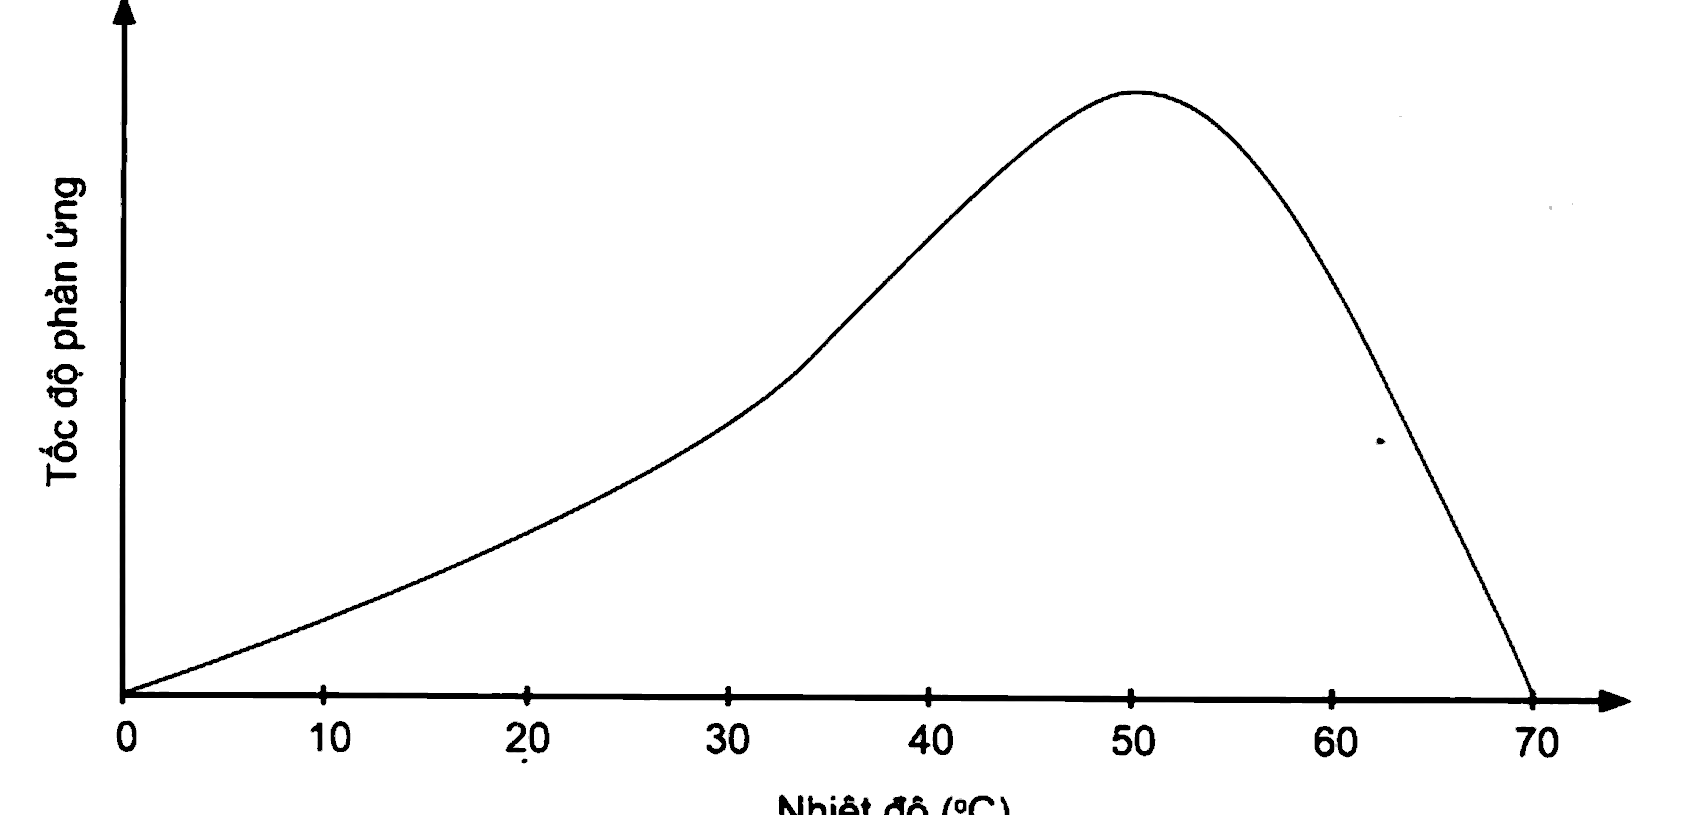
\includegraphics[width=6.5cm]{images_crop_de05/cau14_do_thi_toc_do.png}
\end{center}
Nhiệt độ tối ưu cho enzyme X hoạt động là
\choice
{0$^\circ$C.}
{50$^\circ$C.}
{60$^\circ$C.}
{70$^\circ$C.}
\loigiai{}
\end{ex}

\begin{ex}
(SBT -- CTST). Carbohydrate nào có cấu trúc phân tử được biểu diễn dưới đây?
\begin{center}
	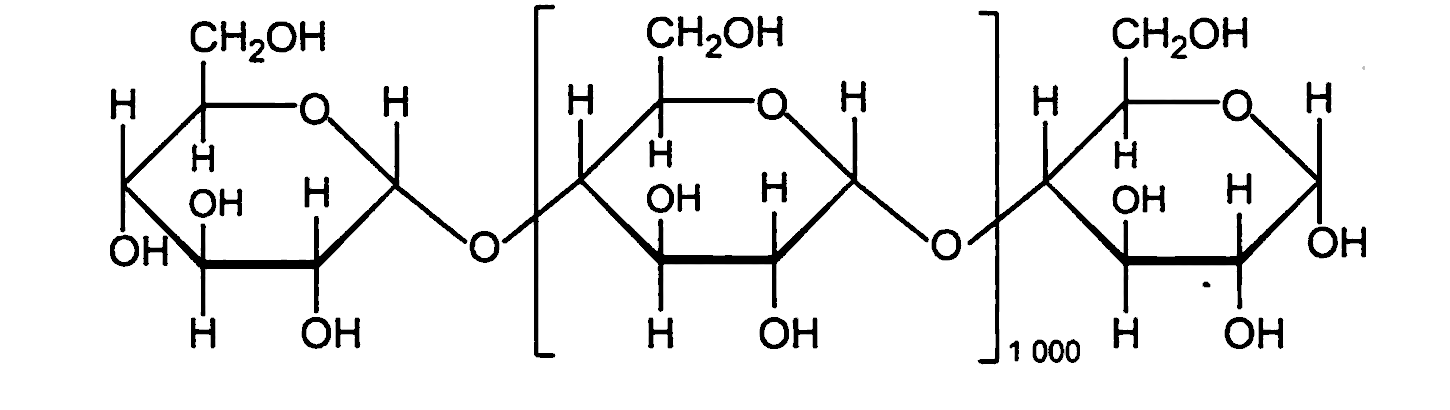
\includegraphics[width=8.5cm]{images_crop_de05/cau15_cau_truc_amylose.png}
\end{center}
\choice
{Saccharose.}
{Cellulose.}
{Maltose.}
{Amylose.}
\loigiai{}
\end{ex}

\begin{ex}
Cho các phát biểu sau về carbohydrate:\\
(a) Tất cả các carbohydrate đều có phản ứng thủy phân.\\
(b) Thủy phân hoàn toàn tinh bột thu được glucose.\\
(c) Glucose, fructose đều có phản ứng tráng bạc.\\
(d) Glucose làm mất màu nước bromine.\\
Số phát biểu đúng là:
\choice
{3.}
{4.}
{1.}
{2.}
\loigiai{}
\end{ex}

\begin{ex}
Cho các phát biểu sau:\\
(a) Đốt cháy hoàn toàn ester no, đơn chức, mạch hở luôn thu được số mol $\ce{CO2}$ bằng số mol $\ce{H2O}$.\\
(b) Trong hợp chất hữu cơ nhất thiết phải có carbon và hydrogen.\\
(c) Những hợp chất hữu cơ có thành phần nguyên tố giống nhau, thành phần phân tử hơn kém nhau một hay nhiều nhóm $\ce{CH2}$ là đồng đẳng của nhau.\\
(d) Dung dịch glucose bị khử bởi $\ce{AgNO3}$ trong $\ce{NH3}$ tạo ra Ag.\\
(e) Saccharose chỉ có cấu tạo mạch vòng.\\
Số phát biểu đúng là
\choice
{4.}
{5.}
{3.}
{2.}
\loigiai{}
\end{ex}

\begin{ex}
Cho các phát biểu sau:\\
(a) Hydrogen hóa hoàn toàn glucose tạo ra acid gluconic.\\
(b) Ở điều kiện thường, glucose và saccharose đều là những chất rắn, dễ tan trong nước.\\
(c) Cellulose trinitrate là nguyên liệu để sản xuất tơ nhân tạo và chế tạo thuốc súng không khói.\\
(d) Amylopectin trong tinh bột chỉ có các liên kết $\alpha$-1,4-glycoside.\\
(e) Saccharose bị hóa đen trong $\ce{H2SO4}$ đặc.\\
(f) Trong công nghiệp dược phẩm, saccharose được dùng để pha chế thuốc.\\
Trong các phát biểu trên, số phát biểu đúng là
\choice
{4.}
{3.}
{2.}
{5.}
\loigiai{}
\end{ex}

\Closesolutionfile{ans}

\vspace{0.15cm}
\noindent
\textbf{PHẦN II (4,0 điểm -- 4 câu): Câu trắc nghiệm đúng sai.}\\
\textit{Thí sinh trả lời từ câu 1 đến câu 4. Trong mỗi ý a), b), c), d) ở mỗi câu, thí sinh chọn đúng hoặc sai.}

\setcounter{ex}{0}

\begin{ex}
(SBT -- KNTT).
\choiceTF[t]
{Tất cả các loại carbohydrate đều tan hoàn toàn trong nước}
{Một số đường đơn (monosaccharide) có vị ngọt}
{Carbohydrate chỉ được tìm thấy trong thực phẩm có nguồn gốc thực vật}
{Glucose và fructose đều là chất rắn, vị ngọt, tan tốt trong nước}
\loigiai{}
\end{ex}

\begin{ex}
Saccharose được tiêu thụ với lượng lớn trên toàn cầu.
\begin{center}
	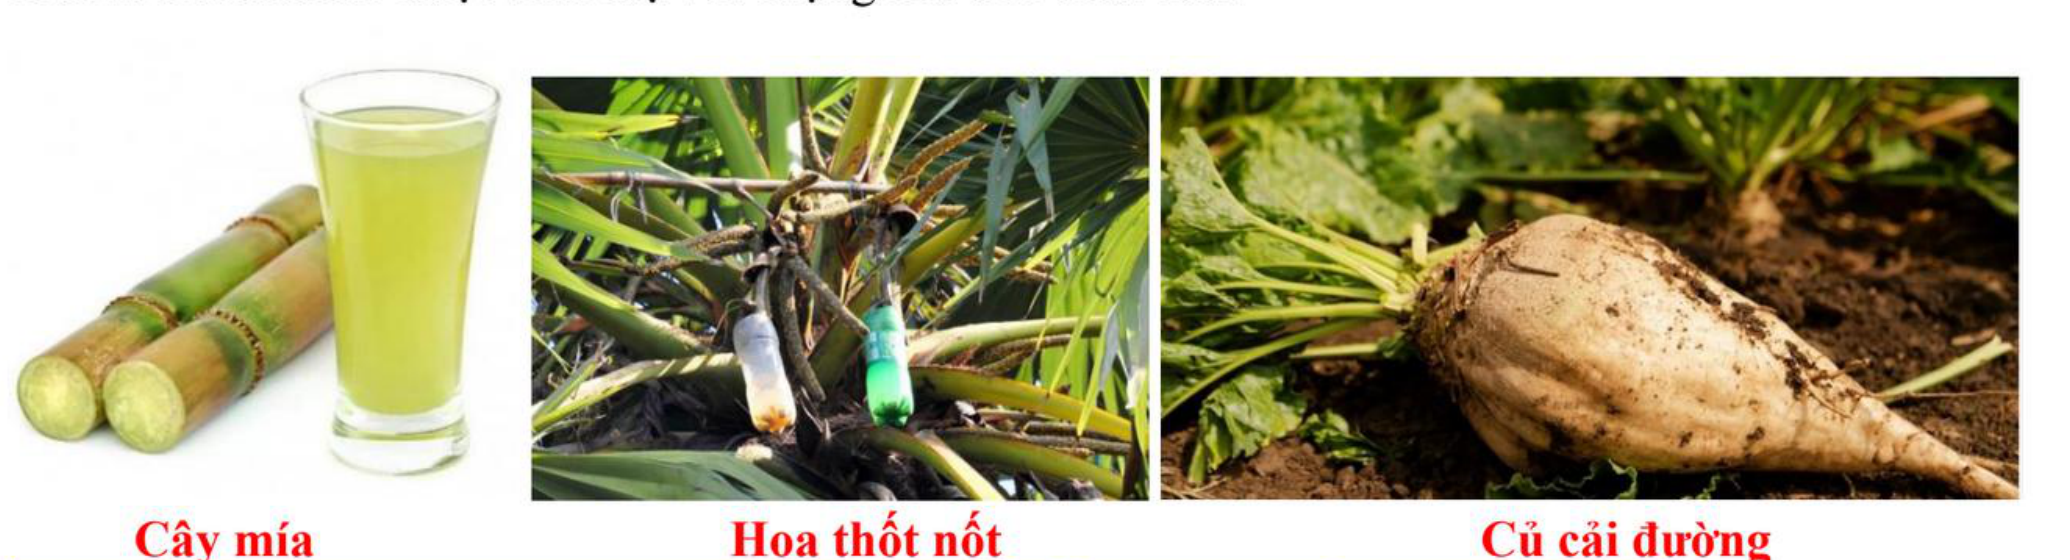
\includegraphics[width=9.5cm]{images_crop_de05/p2_cau2_cay_mia_thot_not_cu_cai.png}
\end{center}
\choiceTF[t]
{Saccharose còn được gọi là đường ăn, là chất rắn, vị ngọt, dễ tan trong nước}
{Saccharose có nhiều trong cây mía, hoa thốt nốt, củ cải đường}
{Thủy phân hoàn toàn saccharose trong môi trường acid chỉ thu được glucose}
{Cấu tạo phân tử saccharose gồm 1 gốc $\alpha$-glucose và 1 gốc $\beta$-fructose liên kết với nhau qua nguyên tử carbon}
\loigiai{}
\end{ex}

\begin{ex}
Cellulose là một polysaccharide gồm nhiều gốc $\beta$-glucose liên kết với nhau tạo ra dạng mạch không nhánh, kéo dài thành dạng sợi có cấu tạo như sau:
\begin{center}
	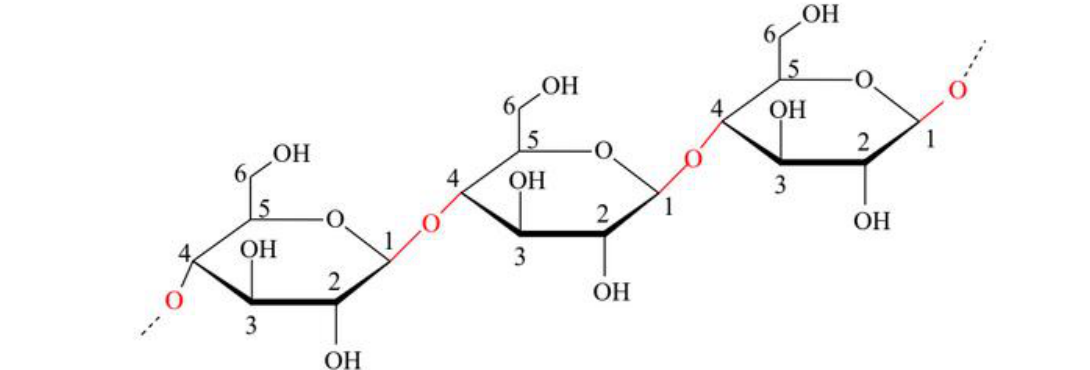
\includegraphics[width=8.5cm]{images_crop_de05/p2_cau3_cau_truc_cellulose.png}
\end{center}
\choiceTF[t]
{Đoạn mạch trên có cả hai loại liên kết là: liên kết $\beta$-1,4-glycoside và liên kết $\beta$-1,6-glycoside}
{Các gốc $\beta$-glucose trong đoạn mạch trên liên kết với nhau bởi liên kết $\beta$-1,4-glycoside}
{Công thức mỗi gốc $\beta$-glucose là $\ce{C6H10O5}$}
{Đoạn mạch trên có cấu tạo phân nhánh ở liên kết $\alpha$-1,6-glycoside}
\loigiai{}
\end{ex}

\begin{ex}
Phản ứng thuỷ phân cellulose trong môi trường acid\\
\textit{Chuẩn bị:}\\
Hoá chất: cellulose (bông), dung dịch $\ce{H2SO4}$ 70\%, dung dịch $\ce{NaOH}$ 10\%, dung dịch $\ce{CuSO4}$ 5\%, $\ce{NaHCO3}$ rắn, nước nóng.\\
Dụng cụ: ống nghiệm, cốc thuỷ tinh 250 mL, đũa thuỷ tinh, đèn cồn, giá đựng ống nghiệm.\\
\textit{Tiến hành:}\\
\textit{Bước 1:} Cho 10 mL dung dịch $\ce{H2SO4}$ 70\% vào cốc thuỷ tinh, thêm một lượng nhỏ cellulose (bông) vào cốc và dùng đũa thuỷ tinh khuấy đều. Sau đó, đặt cốc thuỷ tinh vào cốc nước nóng và khuấy trong khoảng 3 phút để cellulose tan hết tạo dung dịch đồng nhất.\\
\textit{Bước 2:} Trung hoà dung dịch bằng cách thêm từ từ $\ce{NaHCO3}$ đến khi dừng sủi bọt khí, sau đó thêm tiếp 5 mL dung dịch $\ce{NaOH}$ 10\%.\\
\textit{Bước 3:} Cho 5 mL dung dịch thu được ở trên vào ống nghiệm chứa $\ce{Cu(OH)2}$ (được điều chế bằng cách cho 0,5 mL dung dịch $\ce{CuSO4}$ 5\% vào 2 mL dung dịch $\ce{NaOH}$ 10\%, lắc nhẹ). Đun nóng đều ống nghiệm khoảng 2 phút, sau đó để ống nghiệm trên giá khoảng 3 phút.
\choiceTF[t]
{Sau bước 1, sản phẩm thu được có glucose}
{Ở bước 2 thêm từ từ $\ce{NaHCO3}$ để phản ứng diễn ra nhanh hơn}
{Sau bước 3, lấy sản phẩm thu được có kết tủa màu đỏ gạch}
{Thí nghiệm trên chứng minh trong cellulose có thể bị thủy phân trong môi trường acid tạo glucose}
\loigiai{}
\end{ex}

\vspace{0.15cm}
\noindent
\textbf{PHẦN III (1,5 điểm -- 6 câu): Câu trắc nghiệm yêu cầu trả lời ngắn.}\\
\textit{Thí sinh trả lời từ câu 1 đến câu 6. Mỗi câu hỏi thí sinh điền câu trả lời ngắn gọn theo yêu cầu.}

\setcounter{ex}{0}

\begin{ex}
Cho dãy các chất: tinh bột, saccharose, glucose, fructose, cellulose. Số chất trong dãy thuộc loại monosaccharide là bao nhiêu?
\loigiai{}
\noindent\textbf{Đáp số:} \dotfill
\end{ex}

\begin{ex}
Cho các tính chất sau: (1) có vị ngọt, (2) dễ tan trong nước, (3) có phản ứng tráng bạc, (4) bị thủy phân trong môi trường acid, (5) hòa tan $\ce{Cu(OH)2}$ thành dung dịch màu xanh lam. Số tính chất đúng với saccharose là bao nhiêu?
\loigiai{}
\noindent\textbf{Đáp số:} \dotfill
\end{ex}

\begin{ex}
(SBT -- KNTT). Trong số các chất saccharose, maltose, tinh bột và cellulose, có bao nhiêu chất khi thuỷ phân hoàn toàn sản phẩm thu được chỉ là glucose?
\loigiai{}
\noindent\textbf{Đáp số:} \dotfill
\end{ex}

\begin{ex}
Giả thiết phản ứng tổng hợp glucose ở cây lương thực như sau:
\[
\ce{6CO2 + 6H2O} \xrightarrow[\text{chlorophyll}]{\text{asmt}} \ce{C6H12O6 + 6O2} \quad \Delta_r H^\circ_{298} = 2800\text{ kJ}
\]
Trung bình mỗi phút, $1\text{ m}^2$ mặt đất nhận được từ Mặt Trời $60\text{ kJ}$ nhưng chỉ $1\%$ được hấp thụ ở quá trình quang hợp. Khối lượng glucose tổng hợp được trong 7 giờ trên 1 sào ($360\text{ m}^2$) trồng cây lương thực là bao nhiêu gam?
\loigiai{}
\noindent\textbf{Đáp số:} \dotfill
\end{ex}

\begin{ex}
Để tráng bạc (silver) một số ruột phích, người ta phải thuỷ phân $34{,}2\text{ gam}$ saccharose rồi tiến hành phản ứng tráng gương. Có $m\text{ gam}$ Ag tạo thành sau phản ứng, biết hiệu suất mỗi quá trình là $70\%$. Xác định giá trị $m$? (Làm tròn kết quả đến chữ số thập phân thứ nhất).
\loigiai{}
\noindent\textbf{Đáp số:} \dotfill
\end{ex}

\begin{ex}
Xăng E5 được sản xuất bằng cách phối trộn xăng khoáng RON 92 với ethanol ($D = 0{,}8\text{ gam/mL}$) theo tỉ lệ thể tích tương ứng là $95 : 5$. Ethanol được sản xuất từ tinh bột bằng phương pháp lên men. Tinh bột có nhiều trong sắn, ngô. Cho bảng thông tin sau:
\vspace{0.1cm}

\noindent
\begin{minipage}{0.54\textwidth}
\small
\begin{tabular}{|l|c|c|}
\hline
\textbf{Nguyên liệu} & \textbf{Sắn tươi} & \textbf{Ngô khô} \\ \hline
Hàm lượng tinh bột & 30\% & 75\% \\ \hline
Giá 1 kg nguyên liệu & 1.850 đ & 6.500 đ \\ \hline
\end{tabular}
\end{minipage}\hfill
\begin{minipage}{0.44\textwidth}
\centering
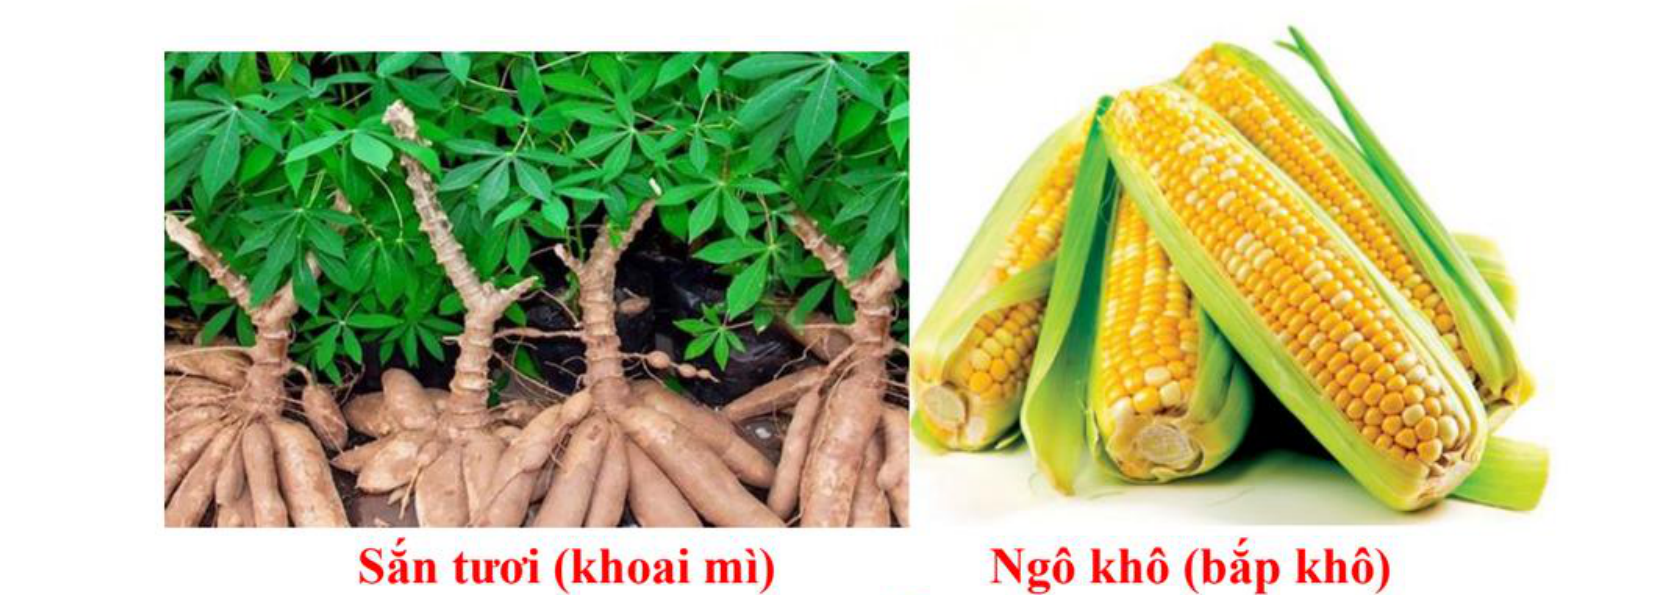
\includegraphics[width=5.5cm]{images_crop_de05/p3_cau6_san_va_ngo.png}
\end{minipage}

\vspace{0.1cm}
Biết hiệu suất của toàn bộ quá trình sản xuất từ sắn tươi đạt $79{,}83\%$, từ ngô khô đạt $84{,}783\%$. Để điều chế $50.000\text{ lít}$ xăng E5 từ sắn tươi cần chi $x$ triệu đồng, từ ngô khô cần chi $y$ triệu đồng. Tính chênh lệch tiền nguyên liệu là $z$ (triệu đồng) khi dùng sắn tươi so với dùng ngô khô để sản xuất. Tính giá trị của $z$ (làm tròn kết quả đến phần triệu).
\loigiai{}
\noindent\textbf{Đáp số:} \dotfill
\end{ex}


\par\vspace{0.1cm}
\centerline{\textbf{---------- HẾT ----------}}

\end{document}
